\documentclass[aspectratio=169]{beamer}

\setbeamersize{text margin left=5mm, text margin right=5mm}

\defbeamertemplate{headline}{my header}{%
\vskip1pt%
\makebox[0pt][l]{\,\insertshortauthor}%
\hspace*{\fill}\insertshorttitle/\insertshortsubtitle\hspace*{\fill}%
\llap{\insertpagenumber/\insertpresentationendpage\,}
}
\setbeamertemplate{headline}[my header]

\let\olditem\item
\renewcommand{\item}{\setlength{\itemsep}{\fill}\olditem}

\usepackage{caption}
\usepackage{soul}
\usepackage{tkz-euclide}
\usetikzlibrary{calc}
\usepackage[]{algorithm2e}
\usepackage{changepage}
\usepackage{amssymb}
\usepackage{bm}
\usepackage{xcolor}
\usepackage{mathtools}
\usepackage{tcolorbox}
\usepackage{tikz}
\usepackage{tikz-3dplot}
\usetikzlibrary{arrows.meta, decorations.pathreplacing, positioning, shapes.geometric}
\usepackage{extarrows}


%% Fonts
\usefonttheme{professionalfonts}
\usefonttheme{serif}

\DeclareCaptionLabelFormat{blank}{}
\captionsetup[figure]{labelformat=blank}

%% Math definitions
\def\mf{\ensuremath\mathbf}
\def\mb{\ensuremath\mathbb}
\def\mc{\ensuremath\mathcal}
\def\lp{\ensuremath\left(}
\def\rp{\ensuremath\right)}
\def\lv{\ensuremath\left\lvert}
\def\rv{\ensuremath\right\rvert}
\def\lV{\ensuremath\left\lVert}
\def\rV{\ensuremath\right\rVert}
\def\lc{\ensuremath\left\{}
\def\rc{\ensuremath\right\}}
\def\ls{\ensuremath\left[}
\def\rs{\ensuremath\right]}
\def\bmx{\ensuremath\begin{bmatrix*}[r]}
\def\emx{\ensuremath\end{bmatrix*}}
\def\bmxc{\ensuremath\begin{bmatrix*}[c]}
\def\t{\lp t\rp}
\def\k{\ls k\rs}

\newcommand{\demoex}[2]{\onslide<#1->\begin{color}{black!60} #2 \end{color}}
\newcommand{\demoexc}[3]{\onslide<#1->\begin{color}{#2} #3 \end{color}}
\newcommand{\anim}[3]{\onslide<#1->{\begin{color}{#2!60} #3 \end{color}}}
\newcommand{\ct}[1]{\lp #1\rp}
\newcommand{\dt}[1]{\ls #1\rs}
\newcommand{\cols}[2]{\begin{columns}[#1] #2 \end{columns}}
\newcommand{\col}[2]{\begin{column}{#1} #2 \end{column}}

%% Mycolors
\definecolor{myred}{RGB}{192,0,0}
\definecolor{mygray}{RGB}{100,100,100}

%% Custom beamer color
\setbeamercolor{title}{fg=myred}
\setbeamercolor{subtitle}{fg=myred}
\setbeamerfont{title}{series=\bfseries}
% \setbeamercolor{frametitle}{bg=myred, fg=white}
\setbeamercolor{frametitle}{bg=mygray!10!, fg=myred}
\setbeamerfont{frametitle}{series=\bfseries}
\setbeamercolor{item}{fg=mygray}
\setbeamercolor{title in head/foot}{fg=myred}

% Move header to footer
\setbeamertemplate{headline}{}
\setbeamertemplate{footline}{
  \begin{beamercolorbox}[wd=\paperwidth,ht=2.25ex,dp=1ex,center]{footline}
    \inserttitle\hfill\insertauthor\hfill\insertdate\hfill\insertframenumber{}
  \end{beamercolorbox}
}

\title{Applied Linear Algebra in Data Analysis}

% A subtitle is optional and this may be deleted
\subtitle{What is this course about?}

\author{Sivakumar Balasubramanian}
% - Give the names in the same order as the appear in the paper.
% - Use the \inst{?} command only if the authors have different
%   affiliation.

\institute[Christian Medical College] % (optional, but mostly needed)
{
  \inst{}%
  Department of Bioengineering\\
  Christian Medical College, Bagayam\\
  Vellore 632002
}
% - Use the \inst command only if there are several affiliations.
% - Keep it simple, no one is interested in your street address.

\date{}
% - Either use conference name or its abbreviation.
% - Not really informative to the audience, more for people (including
%   yourself) who are reading the slides online

\subject{Lecture notes on ALADA}
% This is only inserted into the PDF information catalog. Can be left
% out. 

% If you have a file called "university-logo-filename.xxx", where xxx
% is a graphic format that can be processed by latex or pdflatex,
% resp., then you can add a logo as follows:

% \pgfdeclareimage[height=0.5cm]{university-logo}{university-logo-filename}
% \logo{\pgfuseimage{university-logo}}

% Delete this, if you do not want the table of contents to pop up at
% the beginning of each subsection:
\AtBeginSubsection[]
{
  \begin{frame}<beamer>{Outline}
    \tableofcontents[currentsection,currentsubsection]
  \end{frame}
}

% Let's get started
\begin{document}

\begin{frame}
  \titlepage
\end{frame}


\begin{frame}[t]{What is this course about?}
  \vspace{2cm}
  \begin{center}
    \textcolor{myred}{\huge \textbf{This is an introductory course of high dimensional thinking.}}
  \end{center}
\end{frame}


\begin{frame}[t]{The world is multidimensional}
\begin{itemize}
  \item Most things/systems/ideas of interest in science and engineering are multidimensional.
  \item Undergraduate engineering programs focus on mathematical skills for representing, analysing, and designing relatively simple systems $\longrightarrow$ Univariate \textbf{Calculus}!
  \begin{itemize}
    \item Linear single-input-single-output (SISO) system theory (used in signal processing and control theory).
    \item Fourier, Laplace, z-transforms for understanding 1D temporal or spatial phenomena.
    \item Study of dynamics in mechanical engineering.
  \end{itemize}
  \item Most applications or systems we deal with have multiple degree-of-freedom, various causes and effects, multiple inputs and outputs, multiple measurements, multiple parameters etc.
  \item Dealing with such multidimensional problems requires an additional set of mathematical tools and a different way of thinking. 
\end{itemize}
\end{frame}


\begin{frame}{The world is also uncertain}
\begin{itemize}
  \item Noise and uncertainty are inherent in the real world.
  \item All measurements are corrupted by unwanted sources and the outcomes of all our actions are also influenced by a variety of factors.
  \item There is often some structure to this uncertainty, which can be exploited.
  \item Dealing with uncertainity too requires an additional set of mathematical and statistical tools.
\end{itemize}
\end{frame}


\begin{frame}{We are often faced with multiple options}
\begin{itemize}
  \item There are multiple options for solving a problem. For example,
  \begin{itemize}
    \item Choosing the inputs to a system to get a desired output. 
    \item Estimating a parameter from a set of measurements.
    \item Choose the design parameters for a given set of specifications.
  \end{itemize}
  \vspace{0.2cm}
  \item In such situations, we need to search through the \textit{options space} to find the ``best'' one.
  \vspace{0.2cm}
  \item Various mathematical tools exist for formulating and efficiently solving a wide range of problems.
\end{itemize}
\end{frame}

\begin{frame}{Three major topics are covered in this course}
  \begin{Large}
    {\textbf{Linear Algebra}}
  \end{Large}
  \begin{itemize}
    \item First step in high dimensional thinking.
  \end{itemize}
  \vspace{0.75cm}
  
  \begin{Large}
    {\textbf{Probability theory}}
  \end{Large}
  \begin{itemize}
    \item Principled approach to navigate uncertainity.
  \end{itemize}
  \vspace{0.75cm}
  
  \begin{Large}
    {\textbf{Optimization}}
  \end{Large}
  \begin{itemize}
    \item Approaches for searching spaces for the best solutions.
  \end{itemize}
\end{frame}


\begin{frame}[t]{Linear Algebra}
  \begin{itemize}
    \item Algebra (Arabic: \textit{al-jabr} `reunion of broken parts') is the study of variables and the rules for manipulating these variables in formulas (Source: Wikipedia).
    
    \item Linear algebra is the study of linear system of equations.
    \[
      \left. \begin{aligned}
        a_{11} x_1 + a_{12} x_2 + a_{13} x_3 &+ \cdots + a_{1n} x_n = y_1\\
        &\vdots \\ 
        a_{m1} x_1 + a_{32} x_2 + a_{m3} x_3 &+ \cdots + a_{mn} x_n = y_m
      \end{aligned} \right\} \longrightarrow \mf{A}\mf{x} = \mf{y}
    \]
    These are useful in a surprisingly wide range of real world problems!
    \[ 
      \begin{split}
        x_1, x_2, \ldots x_n &: \text{inputs/parameters of the problem}\\
        y_1, y_2 \ldots y_m &: \text{outputs or measurements}\\
        a_{ij} &: \text{physics of the problem}
      \end{split}
    \]
    \item Linear algebra provides tools for: understanding, manipulating, and efficiently solving such problems.
  \end{itemize}
\end{frame}


\begin{frame}{Probability Theory}
  \begin{itemize}
    \item Branch of mathematics dealing with probability - a measure of uncertainty of events.
    
    \item Provides the tools for representing, analysing, and manipulating uncertainity of events.
    
    \item Some essential concepts: probability distributions/densities, random variables, expectation, variance, covariance, conditional probability, Bayes rule, etc.
    
    \item We will also look at the Gaussian or Normal distribution, arguably the most important distribution in statistics.
  \end{itemize}
\end{frame}


\begin{frame}{Mathematical Optimization}
  \begin{itemize}
    \item Mathematical optimization/programming is the selection of a best element, with regard to some criterion, from a some set of available alternatives. (Source: Wikipedia)
    
    \item We will deal only with continuous optimization problems, where involves searching over the spaces of real numbers $\ct{\mb{R}^n}$.
    
    \item Criteria for choosing the best element is often expressed as a function $\ct{f\ct{\mf{x}}}$ of the elements from the search space $\mb{R}^n$.
    \[ \min_{\mf{x} \in \mb{R}^n} f\ct{\mf{x}} \quad \quad \mathrm{subject \,\, to} \,\, g_i\ct{\mf{x}} \leq 0, \,\, i = 1, \ldots, m \]
  \end{itemize}
\end{frame}
  

\begin{frame}{What kind of problems can we solve with these tools?}
  \begin{columns}
    \begin{column}{0.3\textwidth}
      \begin{itemize}
        \item Signal processing
        \item Control theory
        \item Robotics
        \item Statistics
        \item Machine learning
        \item Medicine
        \item Economics
        \item $\cdots$
      \end{itemize}
    \end{column}
    \begin{column}{0.675\textwidth}
      \begin{figure}
        \centering
        \includegraphics[width=0.8\textwidth]{toomany.png}
      \end{figure}
    \end{column}    
  \end{columns}
\end{frame}


\begin{frame}{Signal Processing}
  We often deal with temporal signal that can be visualized as a function of time. Is this the only way to represent a signal?
  \vspace{0.2cm}

  A sinusoidal signal's time domain representation is shown below. We don't need the signal's entire time record to covney its information. We only need three numbers - the amplitude, frequency, and phase of the sinusoid. These are sufficient to reconstruct the signal. They can be obtained by Fourier transforming the signal into the frequency domain, i.e. a different perspective of the signal.
  \begin{figure}
    \centering
    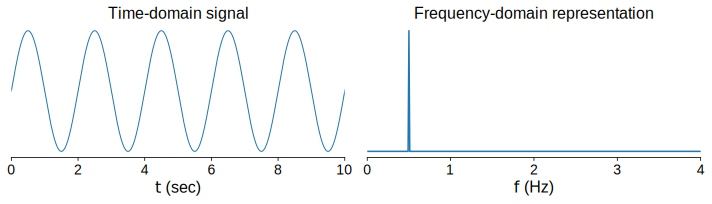
\includegraphics[width=0.8\textwidth]{../../analysis/signalprocessing/output/signal1_fft.png}
  \end{figure}
\end{frame}


\begin{frame}{Signal Processing}
  \begin{itemize}
    \item Expressing signals as a linear combinations of other signals (basis functions) is at the core of most of signal processing.
    \[ x\ct{t} = c_1 \phi_1\ct{t} + c_2 \phi_2\ct{t} + \cdots + c_n \phi_n\ct{t} \]

    \item $\lc c_i \rc_{i}$ is another representation of the signal $x\ct{t}$ in terms of $\lc \phi_i\ct{t} \rc_i$.
    
    \item The Fourier transform is one such representation of a signal.
    
    \item $\lc \phi_i \rc_{i}$ are called the basis functions. Different basis functions gives different types of transforms.
    
    \item Manipulating $\lc c_i \rc_i$ will allow us to extract or suppress different types of information from $x\ct{t}$.
  \end{itemize}
\end{frame}


\begin{frame}{Signal Processing}
  \begin{figure}
    \centering
    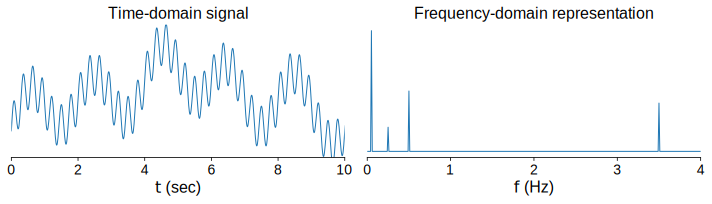
\includegraphics[width=1\textwidth]{../../analysis/signalprocessing/output/signal2_fft.png}
  \end{figure}
\end{frame}


\begin{frame}{Signal Processing}
  \begin{figure}
    \centering
    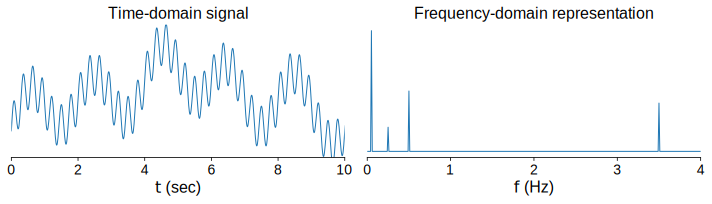
\includegraphics[width=0.8\textwidth]{../../analysis/signalprocessing/output/signal2_fft.png}
  \end{figure}

  What is so special about the Fourier transform? Are there other transforms that might be better suited for certain types of signals? Can I design my own transform?
  \vspace{0.2cm}

  Thinking of signals and images as entities residing in a high-dimensional space turns out to be very useful way to think about signals and how to process them.
\end{frame}


\begin{frame}{Control theory}
  \begin{columns}
    \begin{column}{0.5\textwidth}
      \vspace{0.2cm}
      A spacecraft has 6 DOF - 3 translational $x, y, z$ and 3 rotational $\phi_1, \phi_2, \phi_3$.

      We need both position and velocity information to control the spacecraft.
      \vspace{0.2cm}
      
      The spacecraft has multiple sensors that measure position and velocity.
      \vspace{0.2cm}
      
      Multiple thrusters, reaction-wheels are used to control the spacecraft dynamics.
      \vspace{0.2cm}

      How do we get the best estimate of the spacecraft position and velocity? Which and by how much do we activate the different thrusters and reaction-wheels to control the spacecraft?
    \end{column}
    \begin{column}{0.475\textwidth}
      \begin{figure}
        \centering
        \includegraphics[width=0.9\textwidth]{spacecraft.png}
        \caption{\scriptsize Source: http://surl.li/klulx}
      \end{figure}
    \end{column}    
  \end{columns}
\end{frame}


\begin{frame}{Robotics}
  \begin{columns}
    \begin{column}{0.475\textwidth}
      \begin{figure}
        \centering
        \includegraphics[width=0.825\textwidth]{rehabrobots.png}
        \caption{\scriptsize \textbf{Rehab Robot} [Source: http://surl.li/klupd]}
      \end{figure}
    \end{column}
    \begin{column}{0.5\textwidth}
      \begin{figure}
        \centering
        \includegraphics[width=1\textwidth]{surgicalrobot.png}
        \caption{\scriptsize \textbf{Surgical Robot} [Source: http://surl.li/klurm]}
      \end{figure}
    \end{column}    
  \end{columns}
\end{frame}

\begin{frame}{Robotics}
  \begin{columns}
    \begin{column}{0.5\textwidth}
      Kinematics and dynamics of serial robots are highly non-linear.

      \textbf{Kinematics of a 2-link planar robot}
      \[ 
        \begin{split}
          x &= l_1 \cos\ct{\theta_1} + l_1 \cos\ct{\theta_1 + \theta_2} \\
          y &= l_1 \sin\ct{\theta_1} + l_1 \sin\ct{\theta_1 + \theta_2} \\
        \end{split}
      \]

      The differential kinematics however has is linear relationship:
      \[ \bmx \dot{x} \\ \dot{y}\emx = \mf{J}\ct{\theta_1, \theta_2} \bmx \dot{\theta}_1 \\ \dot{\theta}_2 \emx \]
      \[ \mf{J}\ct{\theta_1, \theta_2}: \text{Jacobian matrix} \]
    \end{column}
    \begin{column}{0.45\textwidth}
      \begin{figure}
        \centering
        \includegraphics[width=0.8\textwidth]{2links.png}
      \end{figure}
    \end{column}    
  \end{columns}
\end{frame}


\begin{frame}{Robotics}
  \begin{columns}
    \begin{column}{0.5\textwidth}
      \textbf{Dynamics of serial robots.}
      \[ 
        \mf{M}\ct{\mf{q}} \ddot{\mf{q}} + \mf{C}\ct{\mf{q}, \dot{\mf{q}}} \dot{\mf{q}} + \mf{g}\ct{\mf{q}} = \bm{\tau} + \mf{J}^\top \mf{f}
      \]
      where,
      \begin{itemize}
        \item $\mf{q}$: Joint angles
        \item $\mf{M}\ct{\mf{q}}$: Inertia matrix
        \item $\mf{C}\ct{\mf{q}, \dot{\mf{q}}}$: Coriolis and centrifugal forces
        \item $\mf{g}\ct{\mf{q}}$: Gravity forces
        \item $\bm{\tau}$: Joint torques
      \end{itemize}
      
    \end{column}
    \begin{column}{0.45\textwidth}
      \begin{figure}
        \centering
        \includegraphics[width=0.8\textwidth]{2links.png}
      \end{figure}
    \end{column}    
  \end{columns}
\end{frame}


\begin{frame}{Statistics}
  The data that we deal with is often heterogeneous, high-dimensional, and noisy.
  \vspace{1cm}
  
  \textbf{Core of statistics:}
  \begin{itemize}
    \item Representing such data
    \item Evaluating the relationships between different variables
    \item Building and estimating models for inference and decision making
  \end{itemize}
  \vspace{1cm}
  
  Proability theory, Calculus, Linear algebra, and Optimiztion are employed for solving these problems efficiently.
\end{frame}


\begin{frame}{Statistics}
  Health-related physical fitness (HRPF) can be good indicator for the developments of chronic diseases [1].

  HRPF can be difficult to measure and has multiple components - HGS, STS, and $VO_2$ max.
  
  Can we predict these HRPF component's from easily measurable variables -- age, height, weight, BMI, and \% body fat?

  \[ y_j = \beta_0 + \beta_1 x_{j1} + \beta_2 x_{j2} + \cdots + \beta_n x_{jn} + \epsilon_j \,\, \longrightarrow \,\, \mf{y} = \mf{X}\bm{\beta} + \bm{\epsilon} \]
  \[ \min_{\bm{\beta}} \Vert \mf{y} - \mf{X}\bm{\beta}\Vert_2^2 \implies \hat{\bm{\beta}} = \lp \mf{X}^\top{\mf{X}} \rp^{-1}\mf{X}^\top\mf{y} \]

  \vspace{0.75cm}

  \begin{small}
    [1] Kim, S.-W. et al., Front. Physiol. 12, 668055 (2021).
  \end{small}
\end{frame}


\begin{frame}{Statistics}
  What if we want to have a minimalistic model --  good performance with fewest number of variables?
  \[ \mf{y} = \mf{X}\bm{\beta} + \bm{\epsilon} \]

  \textbf{Ridge Regression:}
  \[ \min_{\bm{\beta}} \Vert \mf{y} - \mf{X}\bm{\beta}\Vert_2^2 + \lambda \Vert \bm{\beta} \Vert_2^2 \implies \hat{\bm{\beta}} = \lp \mf{X}^\top{\mf{X}} + \lambda \mf{I} \rp^{-1}\mf{X}^\top\mf{y} \]

  \vspace{0.7cm}

  \textbf{LASSO Regression:}
  \[ \min_{\bm{\beta}} \Vert \mf{y} - \mf{X}\bm{\beta}\Vert_2^2 + \lambda \Vert \bm{\beta} \Vert_1 \]
\end{frame}


\begin{frame}{Machine learning}
  In machine learning, we are interested in modelling complex models through the use of data.
  \vspace{0.5cm}
  
  Data is almost always high dimensional in such applications with complex structure.
  \vspace{0.5cm}
  
  Models we are interested in fitting a more complex than linear models.
  \begin{itemize}
    \item Linear/Logistic Regression
    \item Decision trees, random forests
    \item Support vector machines
    \item Neural networks
    \item $\cdots$
  \end{itemize}
\end{frame}


\begin{frame}{Why do this course?}
  \begin{center}
    \textcolor{myred}{\huge \textbf{This is will prepare you to comfortably work with such problems.}}
  \end{center}
\end{frame}


\end{document}